\documentclass[10pt,a4paper]{article}
\usepackage[margin=20mm]{geometry}
\usepackage{amsmath,amssymb,booktabs,graphicx,tabularx,array}
\usepackage[T1]{fontenc}
\usepackage{lmodern,microtype,xcolor}
\usepackage{enumitem,float,placeins}
\usepackage{tikz}
\usetikzlibrary{arrows.meta,positioning}
\newcounter{workflowdiagram}
\usepackage[colorlinks=true,linkcolor=blue!45!black,urlcolor=blue!45!black,citecolor=blue!45!black]{hyperref}
\setlist{itemsep=2pt,topsep=4pt}
\setlength{\parindent}{0pt}
\setlength{\parskip}{4pt}
\setlength{\textfloatsep}{10pt plus 2pt minus 2pt}
\setlength{\floatsep}{8pt plus 2pt minus 2pt}
\setlength{\intextsep}{10pt plus 2pt minus 2pt}
\renewcommand{\topfraction}{0.9}
\renewcommand{\bottomfraction}{0.85}
\renewcommand{\textfraction}{0.08}
\renewcommand{\floatpagefraction}{0.8}
\raggedbottom
\setcounter{tocdepth}{1}
\emergencystretch=2em
\brokenpenalty=10000
\graphicspath{{../results/figures/}}
\newcommand{\RunSeconds}{5.97}
\newcommand{\LaplaceAcc}{97.69}
\newcommand{\LaplaceNLL}{0.151}
\newcommand{\MapNLL}{0.099}
\newcommand{\E}{\mathbb{E}}
\newcommand{\R}{\mathbb{R}}
\title{\textbf{Bayesian Handwritten Digit Recognition}\\
Last-Layer Laplace Inference with an Exact Conditional Hessian}
\author{Paco, Sou Chak Tong\\Student ID: U-C3-2652-3\\
CISC3024 --- Pattern Recognition\\AI Assignment \#2}
\date{8 October 2026}
\begin{document}
\maketitle
\begin{abstract}
This coursework implements a small-scale last-layer Laplace classifier motivated by
\emph{Laplace Redux} (NeurIPS 2021). A learned image representation is frozen,
a Gaussian prior is placed over its linear classification head, and an exact
conditional softmax Hessian defines a Gaussian approximation to the posterior.
Predictions average class probabilities over 512 sampled heads. The study uses
1,797 handwritten digit images, a fixed stratified split of 1,077/360/360 images,
and three independent neural initialization seeds. Validation selects checkpoints
and prior precision before final test prediction. Laplace achieves
\LaplaceAcc\% mean accuracy and \LaplaceNLL\ mean negative log-likelihood (NLL).
A separately selected maximum a posteriori (MAP) classifier has lower NLL
(\MapNLL). A frozen-prior ablation confirms that posterior averaging reduces
probability quality here, while dropping posterior correlations reduces it further.
Thus Bayesian inference provides explicit uncertainty, but does not guarantee
better calibration. The AI agent performed research, programming, experiments and
report drafting; the personal reflection remains student-authored.
\end{abstract}
\textbf{Scope.} This is an independently coded, educational adaptation of a
recent practical Bayesian framework, not a reproduction of its published
benchmark results. All numerical results come from this project's saved
outputs. Public publication is deliberately deferred to Prompt 03.
\tableofcontents
\clearpage

\section{How AI Found the Algorithm}
\subsection{How the student structured Codex's work}
The student guided Codex Desktop through a hierarchy of written instructions.
The instructor's \texttt{AIassign2.pdf} defined the assignment: a recent
probability- or Bayes-based recognition algorithm, AI-written technical code and
six required report items. Codex extracted the complete one-page PDF and
inspected its rendering. The project \texttt{AGENTS.md} supplied persistent
rules for scientific integrity, reproducibility, mathematical rigor, held-out
evaluation and student authorship. Task-specific Markdown prompts supplied the
executable stages; installed skills supplied procedural guidance for carrying
out those stages. The project priority was course requirements, then
\texttt{AGENTS.md}, then the current task prompt, then skill guidance.

The student explicitly invoked Prompt 01 for research, implementation,
experiments and reporting, then Prompt 02 for technical and figure review.
Later requests refined the report and supplied the student's own reflection.
Workflow diagram~\ref{fig:ai-workflow} distinguishes these executed activities
from the deferred publication and post-publication audit. Descriptions below
are evidence-based paraphrases; only the quotation column reproduces prompt text.
% Vector workflow; independent caption counter preserves experimental figure numbering.
\begin{figure}[H]
\centering
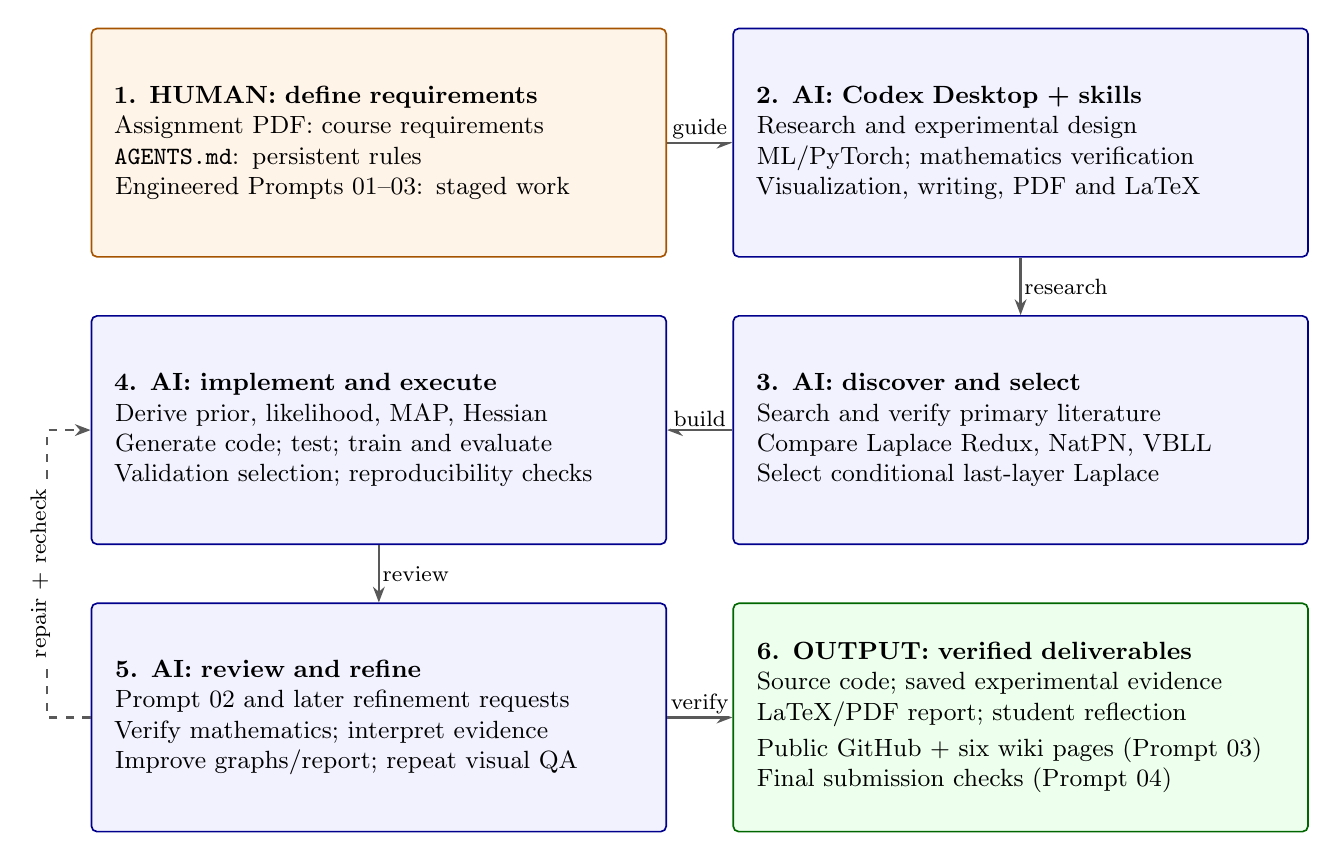
\begin{tikzpicture}[
  box/.style={draw=black!55,rounded corners=2pt,line width=.6pt,
    text width=67mm,minimum height=29mm,inner sep=3mm,
    align=left,font=\fontsize{9}{11}\selectfont},
  human/.style={box,fill=orange!9,draw=orange!65!black},
  activity/.style={box,fill=blue!5,draw=blue!55!black},
  output/.style={box,fill=green!7,draw=green!40!black},
  flow/.style={-{Stealth[length=2mm]},line width=.8pt,draw=black!65},
  edge/.style={font=\fontsize{8}{9}\selectfont,fill=white,inner sep=1pt}
]
\node[human] (human) at (0,0) {\textbf{1. HUMAN: define requirements}\\
  Assignment PDF: course requirements\\
  \texttt{AGENTS.md}: persistent rules\\
  Engineered Prompts 01--03: staged work};
\node[activity] (agent) at (8.15,0) {\textbf{2. AI: Codex Desktop + skills}\\
  Research and experimental design\\
  ML/PyTorch; mathematics verification\\
  Visualization, writing, PDF and LaTeX};
\node[activity] (discovery) at (8.15,-3.65) {\textbf{3. AI: discover and select}\\
  Search and verify primary literature\\
  Compare Laplace Redux, NatPN, VBLL\\
  Select conditional last-layer Laplace};
\node[activity] (execute) at (0,-3.65) {\textbf{4. AI: implement and execute}\\
  Derive prior, likelihood, MAP, Hessian\\
  Generate code; test; train and evaluate\\
  Validation selection; reproducibility checks};
\node[activity] (review) at (0,-7.3) {\textbf{5. AI: review and refine}\\
  Prompt 02 and later refinement requests\\
  Verify mathematics; interpret evidence\\
  Improve graphs/report; repeat visual QA};
\node[output] (deliver) at (8.15,-7.3) {\textbf{6. OUTPUT: verified deliverables}\\
  Source code; saved experimental evidence\\
  LaTeX/PDF report; student reflection\\[2pt]
  Public GitHub + six wiki pages (Prompt 03)\\
  Final submission checks (Prompt 04)};
\draw[flow] (human.east) -- node[edge,above]{guide} (agent.west);
\draw[flow] (agent.south) -- node[edge,right]{research} (discovery.north);
\draw[flow] (discovery.west) -- node[edge,above]{build} (execute.east);
\draw[flow] (execute.south) -- node[edge,right]{review} (review.north);
\draw[flow] (review.east) -- node[edge,above]{verify} (deliver.west);
\draw[flow,dashed] (review.west) -- ++(-.55,0) |- (execute.west);
\node[edge,rotate=90] at (-4.3,-5.47) {repair + recheck};
\end{tikzpicture}
\par\smallskip
\refstepcounter{workflowdiagram}\label{fig:ai-workflow}
{\small\textbf{Workflow diagram \theworkflowdiagram.}
Human instructions (orange), AI activities (blue) and generated outputs (green).
Arrows trace executed work; the dashed loop denotes repair and rechecking.
Repository, wiki and final submission checks are verified.
Skill contributions and limits are identified in the accompanying text.}
\end{figure}


\textbf{What the skills actually contributed.}
The usage record identifies \texttt{literature-review} for primary-source
provenance; \texttt{experimental-design} for matched controls and seed replication;
and \texttt{scikit-learn} for splitting, baselines and metric conventions.
Machine-learning, \texttt{pytorch-patterns} and \texttt{pytorch-training-recipe}
guidance informed deterministic training, device handling and checkpoint checks.
\texttt{scientific-visualization} informed scales, sample counts, vector exports
and final-size readability. PDF guidance supported extraction/rendering, while
the LaTeX compile plugin provided compiler detection and actual builds.
These were procedural aids, not experimental evidence \cite{skills}.

\texttt{scientific-writing} and \texttt{latex-paper-en} were inspected in
Prompt 01, but their review services/scripts were not used then. Prompt 02
materially applied their writing, caption and reviewer guidance, together with
\texttt{statistical-analysis} for replication units and uncertainty interpretation.
Installed \texttt{pymc}, \texttt{exploratory-data-analysis},
\texttt{analytical-method-validation} and \texttt{markdown-mermaid-writing} have
no documented material role and are not credited as used. No subagent,
paid schematic generator or external manuscript-review service was used.
\clearpage

\subsection{Verified instructions and their executed responses}
P01 denotes \path{prompts/01_RESEARCH_IMPLEMENT_REPORT.md};
P02 denotes \path{prompts/02_CRITICAL_REVIEW_AND_FIGURES.md}.
A, C and D identify the named phases in P01; QA3 is step 3 of P02's required
QA loop. Each row gives a verbatim extract, its purpose and the recorded response.
The comparison extract begins mid-sentence; none of the extracts is a fabricated
conversation or a claim that every available skill was invoked.
\begin{table}[H]\centering
\fontsize{9}{11}\selectfont
\setlength{\tabcolsep}{4pt}
\renewcommand{\arraystretch}{1.15}
\begin{tabularx}{\linewidth}{>{\raggedright\arraybackslash}p{19mm}>{\raggedright\arraybackslash}p{67mm}>{\raggedright\arraybackslash}X}
\toprule Source & Verbatim instruction & Purpose and actual response\\
\midrule
P01/D & ``Use only verified citations.'' & \textbf{Source verification.} Primary proceedings/manuscripts supplied metadata; queries and source URLs were recorded, and all eight references were rechecked in Prompt 02. \\
P01/A & ``and compare: publication/year, mathematical basis, relevance to the course, reproducibility, compute/data requirements, evaluation protocol, and risk.'' & \textbf{Substantive comparison.} Codex compared Laplace Redux, NatPN and VBLL on these criteria before implementing conditional Laplace. \\
P01/A & ``Prefer genuinely recent publications (approximately 2021--2026) while citing older foundational Bayesian/probabilistic work when appropriate.'' & \textbf{Honest recency.} The report identifies the 2021 choice as the older edge of this range, explains its practical contribution and treats MacKay as foundational background. \\
P01/A & ``Verify important symbolic or numerical identities against the implementation.'' & \textbf{Mathematical accountability.} Analytic gradients/Hessians were checked against autograd; covariance sampling, normalization and a two-class example were tested. \\
P01/C & ``Use a proper train/validation/test strategy; select models with validation only.'' & \textbf{Leakage prevention.} Saved split indices and selection records document validation-based checkpoint/prior choice before final test prediction, with three neural seeds. \\
P02/QA3 & ``Re-run affected tests, figure generation, experiments where necessary, and bibliography/reference checks.'' & \textbf{Repair with evidence.} The loss-logging repair was tested and reproduced; nine tests passed, 18 primary arrays stayed identical, and citations were rechecked. \\
P02/Figures & ``Use a controlled layout with informative whitespace; no unnecessary pages or enormous gaps.'' & \textbf{Final-size readability.} Codex enlarged labels, redesigned reliability/uncertainty displays and inspected exports on rendered report pages; later refinement corrected bounded F1 presentation. \\
\bottomrule
\end{tabularx}
\caption{Selected instructions verified against the original prompt files.
Responses are summaries of saved research, implementation and review records.}
\end{table}

\textbf{Recorded discovery queries (8 October 2026).}
The research log retains these actual algorithm-search strings:
\begin{itemize}[leftmargin=12pt,itemsep=1pt,topsep=2pt]
\item \emph{Laplace Redux Effortless Bayesian Deep Learning NeurIPS 2021 Daxberger}
\item \emph{Posterior Network uncertainty estimation without OOD samples NeurIPS 2020 Natural Posterior Network 2021}
\item \emph{2022 Bayesian neural network classification variational inference last layer uncertainty paper}
\end{itemize}
The second query includes an older Posterior Network search term; the candidate
actually compared was Natural Posterior Network (ICLR 2022). Additional recorded
queries targeted Guo's calibration paper and MacKay's Bayesian interpolation
paper for background, rather than treating them as recent candidate methods.

\textbf{Verification and scope.}
Codex opened primary proceedings, author manuscripts and dataset documentation,
checking titles, authors, venues/years and available DOI/page metadata.
Laplace's NeurIPS proceedings/PDF, NatPN's ICLR PDF/arXiv manuscript and VBLL's
ICLR PDF/arXiv record supplied the candidate evidence. OpenReview forum pages
returned a verification challenge and a NeurIPS BibTeX link returned a tool
error; accessible primary PDFs/records supplied the missing metadata.
This was a bounded narrative search, not an exhaustive systematic review.
Verification was by the AI agent, not an independent human reviewer.
\clearpage

\subsection{Candidate comparison and final selection}

\begin{table}[H]\centering\small
\begin{tabularx}{\linewidth}{>{\raggedright\arraybackslash}p{25mm}>{\raggedright\arraybackslash}p{20mm}>{\raggedright\arraybackslash}X>{\raggedright\arraybackslash}X}
\toprule Method & Publication & Defining probability mechanism & Feasibility and main risk\\
\midrule
Laplace Redux & NeurIPS 2021 & Gaussian approximation around MAP; posterior integration &
Post-hoc head inference is tractable; a local Gaussian can misrepresent uncertainty.\\
Natural Posterior Network & ICLR 2022 & Density-dependent conjugate updates for exponential-family targets &
Learned features and normalizing flows; density training adds complexity and failure modes.\\
Variational Bayesian Last Layers & ICLR 2024 & Deterministic variational formulation for Bayesian output layers &
Efficient last-layer training; its variational objective adds implementation work.\\
\bottomrule
\end{tabularx}
\caption{Candidate methods verified from primary sources \cite{laplace,natpn,vbll}.
All address probabilistic prediction and can be evaluated on image recognition.}
\end{table}
\textbf{Why Laplace Redux rather than a newer method?}
The original choice prioritized an auditable probability model and controlled
approximation comparisons. Section 2 of Laplace Redux separates the uncertain
weight subset, curvature structure, prior selection and predictive integration
\cite{laplace}. These choices directly support this study's fixed-feature,
matched-MAP and diagonal-precision controls. With only 330 head parameters,
the complete conditional Hessian can be derived, stored and checked against
autograd; linear head logits also make the conditional Hessian equal to the
generalized Gauss--Newton curvature. This gives a concrete route from prior and
likelihood to a testable posterior calculation.

Newer alternatives remain credible. VBLL offers efficient sampling-free
variational training and explicitly supports frozen-feature post-training
\cite{vbll}; it was not rejected as infeasible. Its learned variational
mean/covariance and bound-based objective would change the inference question
from local curvature at a conditional MAP optimum. NatPN instead converts learned
feature densities into conjugate posterior updates \cite{natpn}, adding a density
estimation mechanism suited to a different uncertainty study. The preference
here is mathematical inspectability, not an empirical claim that these methods
are less accurate or less calibrated; neither was run in this project.

The 2021 paper is at the older edge of the requested 2021--2026 range. Its recent
contribution is a practical framework/library and evaluation, not the invention
of Bayes or Laplace theory \cite{mackay}. This implementation chooses full
curvature, validation tuning and Monte Carlo prediction instead of the paper's
default KFAC, empirical-Bayes and probit choices \cite{laplace}. The justification
therefore supports an educational adaptation, not a state-of-the-art or full
benchmark-reproduction claim, and does not use test outcomes to change the method.


\subsection{How staged review changed the outcome}
Prompt 01 produced an executable study and a first compiled report. Prompt 02
then required section-by-section criticism and repeated visual QA. It strengthened
the distinction between an exact conditional Hessian and an approximate Gaussian
posterior, added a tested two-class covariance example, and corrected the
pre-update training versus post-update validation loss log. Reproduction retained
the primary predictions. A separately recorded post hoc diagnostic executed
72 fixed-model predictions to quantify Monte Carlo integration variation;
it neither selected new models nor turned seed spread into a dataset confidence
interval. The unfavorable probability-quality result was preserved.

The review enlarged confusion labels, separated seed markers, replaced joined
reliability lines with occupied-bin points, and normalized uncertainty displays
within correct/error groups. Later refinement showed bounded F1 deficits as
individual seed values and observed ranges, avoiding a misleading negative
mean-minus-SD endpoint without deleting measurements. It also added covariance
geometry and improved page layout. These were same-agent self-review and
refinement, not independent peer review; Sections 2--4 give the technical detail.

\textbf{Complete records and publication status.}
The source tree preserves \texttt{AGENTS.md}, all four original files in
\texttt{prompts/}, \texttt{docs/research.md}, \texttt{docs/ai\_usage.md},
\texttt{docs/review\_02.md} and \texttt{docs/refinement\_02.md}.
\texttt{docs/skill\_sources.md} identifies the actual skill documents, origins,
local hashes and consultation status. These records and linked complete skill
documentation are intended for the public repository created in Prompt 03;
Section 6 will contain its verified URL after publication. Prompt 03 and
\path{prompts/04_FINAL_SUBMISSION_AUDIT.md} remain pending. No public URL or
completed publication is implied here.

\section{Algorithm Description}
\subsection{Task, notation and conditional model}
An image is an $8\times8$ grayscale array with integer acquisition values from
0 to 16. Flattening gives $x\in[0,1]^{64}$ after division by the fixed maximum
16. Let $y\in\{0,\ldots,9\}$ be its digit label, $K=10$, and
$\mathcal D=\{(x_n,y_n)\}_{n=1}^{N}$ the training partition.
A deterministic neural representation is
\begin{equation}
h_\phi(x)=\tanh(Ax+a)\in\R^{32},\qquad
f_\phi(x)=\begin{bmatrix}h_\phi(x)\\1\end{bmatrix}\in\R^{D},\quad D=33.
\end{equation}
The appended one makes bias parameters part of the same algebra as weights.
A head $W\in\R^{K\times D}$ produces logits $z_k=w_k^\top f_\phi(x)$.
After training the representation, $\phi$ is frozen. Bayesian inference is
\emph{conditional on this learned representation}; it does not infer a
distribution over all network weights.

\begin{table}[H]\centering
\begin{tabular}{ll}\toprule Symbol & Meaning\\\midrule
$N=1077$ & Training images\\
$K=10$, $D=33$ & Classes and augmented feature dimension\\
$\theta=\operatorname{vec}_{\rm row}(W)\in\R^{330}$ & Class-major head parameter vector\\
$\alpha>0$ & Isotropic Gaussian prior precision\\
$H$, $\Sigma$ & Posterior precision Hessian and covariance\\
$S=512$ & Monte Carlo weight draws per prediction run\\
$q(\theta)$ & Gaussian approximation to the conditional posterior\\
\bottomrule\end{tabular}
\caption{Notation matched to array layouts in \texttt{laplace.py}.}
\end{table}

\subsection{Likelihood, prior and posterior}
The defining conditional likelihood is categorical:
\begin{equation}
p(y=k\mid x,W,\phi)=p_k(x;W)
=\frac{\exp(w_k^\top f_\phi(x))}
{\sum_{j=0}^{K-1}\exp(w_j^\top f_\phi(x))}.
\end{equation}
Training observations are modeled as conditionally independent.
An isotropic prior is imposed on \emph{every} head parameter, including biases:
\begin{equation}
p(\theta\mid\alpha)=
\left(\frac{\alpha}{2\pi}\right)^{KD/2}
\exp\left(-\frac{\alpha}{2}\|\theta\|_2^2\right).
\end{equation}
Bayes' rule gives
\begin{equation}
p(\theta\mid\mathcal D,\phi,\alpha)
=\frac{p(\mathcal D\mid\theta,\phi)p(\theta\mid\alpha)}
{\int p(\mathcal D\mid u,\phi)p(u\mid\alpha)\,du}.
\end{equation}
For fixed $\alpha$ and $\phi$, constants independent of $\theta$ can be discarded.
The negative log-posterior objective is therefore
\begin{equation}\label{eq:objective}
L(\theta)=\sum_{n=1}^N
\left[\log\sum_j\exp(w_j^\top f_n)-w_{y_n}^\top f_n\right]
+\frac{\alpha}{2}\|\theta\|_2^2 .
\end{equation}
The implementation uses stable \texttt{logsumexp} and sums the likelihood.
A mean loss with the same numerical $\alpha$ would change the prior's
relative strength by a factor of $N$. Feature training uses a separate
mean cross-entropy and regularizer; its optimizer decay is not
identified with this conditional head prior.


\subsection{MAP estimation and exact curvature}
For fixed features, the objective is convex. A strictly positive prior precision
makes it strictly convex, with a unique head optimum
$\hat\theta=\arg\min_\theta L(\theta)$.
Let $t_{nk}=\mathbb{1}\{y_n=k\}$. Differentiating the normalizer gives
$\partial\log\sum_j e^{z_j}/\partial z_k=p_{nk}$, hence
\begin{equation}
\frac{\partial L}{\partial w_k}
=\sum_{n=1}^N(p_{nk}-t_{nk})f_n+\alpha w_k .
\end{equation}
L-BFGS minimizes this objective using an analytic gradient. Every run checks the
optimizer status and requires the maximum absolute summed-objective gradient
component to be below $10^{-3}$. Recorded candidate gradients are much smaller.

Differentiating softmax gives
$\partial p_k/\partial z_l=p_k(\delta_{kl}-p_l)$. Thus the exact Hessian
entries, in the class-major ordering used by the code, are
\begin{equation}\label{eq:hessian}
H_{(k,a),(l,b)}=
\sum_{n=1}^N p_{nk}(\delta_{kl}-p_{nl})f_{na}f_{nb}
+\alpha\delta_{kl}\delta_{ab}.
\end{equation}
Equivalently, with $B_n=\operatorname{diag}(p_n)-p_np_n^\top$,
\begin{equation}
H=\sum_{n=1}^N B_n\otimes(f_nf_n^\top)+\alpha I_{KD}.
\end{equation}
This is the \emph{exact conditional} Hessian for linear logits. It is not an
exact full-network Hessian: nonlinear feature parameters are held fixed.
A generalized Gauss--Newton expression coincides with this Hessian in
the conditional linear-logit case.

For any $v\in\R^K$,
$v^\top B_nv=\sum_kp_{nk}v_k^2-(\sum_kp_{nk}v_k)^2\geq0$:
it is a variance under a categorical distribution. Thus
$H\succeq\alpha I$ and Cholesky factorization is well defined. At $\alpha=0$,
a common-logit shift direction is unidentifiable and curvature is singular.
A proper prior resolves this issue. Nonpositive precisions are rejected
rather than hidden by arbitrary damping.

\subsection{Local Gaussian approximation}
Expand the negative log-posterior near its optimum:
\begin{equation}
L(\theta)\approx L(\hat\theta)+
\underbrace{\nabla L(\hat\theta)^\top(\theta-\hat\theta)}_{\approx0}
+\frac12(\theta-\hat\theta)^\top H(\theta-\hat\theta).
\end{equation}
Exponentiating its negative and normalizing yields
\begin{equation}
q(\theta)=\mathcal N(\hat\theta,H^{-1}),\qquad \Sigma=H^{-1}.
\end{equation}
A Gaussian prior is not conjugate to a categorical softmax likelihood; the true
posterior is generally not Gaussian. The second-order expansion is an
approximation even when its Hessian is exact. The code computes the full
$330\times330$ precision matrix in double precision. No diagonal or Kronecker
curvature approximation is used for the primary method. The small problem
makes its full covariance practical and indexing testable.

\textbf{Worked conditional example.} Consider two classes, one scalar feature
$f=1$, two training observations with labels 0 and 1, and $\alpha=1$.
Symmetry and strict convexity give $\hat W=(0,0)^\top$ and $p=(1/2,1/2)$.
Each observation contributes $B=\frac14\left[\begin{smallmatrix}1&-1\\-1&1\end{smallmatrix}\right]$;
summing both contributions and adding the prior gives
\begin{equation}
H=\begin{bmatrix}1.5&-0.5\\-0.5&1.5\end{bmatrix},\qquad
\Sigma=H^{-1}=\begin{bmatrix}0.75&0.25\\0.25&0.75\end{bmatrix}.
\end{equation}
The probability depends on the logit difference $d=w_1-w_0$, not their
common offset. Its variance is $0.75+0.75-2(0.25)=1$.
Dropping off-diagonal precision first gives covariance $(2/3)I$ and
$\operatorname{Var}(d)=4/3$. Thus the diagonal approximation can increase
\emph{contrast} variance even though each marginal variance decreases.
The common direction $(1,1)$ has curvature 1, supplied solely by the prior;
the contrast direction $(1,-1)$ has curvature 2. A unit test verifies the
MAP, Hessian and both contrast variances. This exact toy calculation illustrates
correlation cancellation; it does not measure the ten-class experiment's mechanism.

\begin{center}
\begin{minipage}{\linewidth}\centering
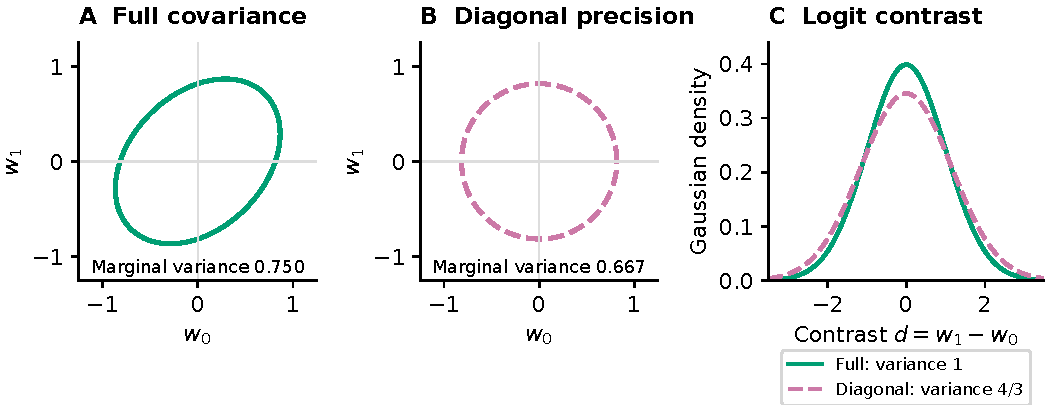
\includegraphics[width=\linewidth]{covariance_geometry.pdf}
\parbox{\linewidth}{\small\textbf{Worked-example geometry (not experimental data).}
Radius-one Mahalanobis contours of the two Gaussian approximations have the same
center. Diagonalizing precision before inversion shrinks marginal variances
from $3/4$ to $2/3$, yet the contrast $w_1-w_0$ becomes wider: variance 1 versus
$4/3$. These contours are not 68\% joint credible regions; the exact Gaussian
contrast densities at right explain why smaller marginal variance need not mean
more certain class probabilities. The contour equation is verified numerically.}
\end{minipage}
\end{center}


\subsection{Posterior predictive classification}
A Bayesian prediction integrates the uncertain head:
\begin{equation}
\bar p_k(x)=\int p_k(x;\theta)q(\theta)\,d\theta
\approx \frac1S\sum_{s=1}^S p_k(x;\theta^{(s)}),\qquad
\hat y(x)=\arg\max_k\bar p_k(x).
\end{equation}
Let $H=LL^\top$ with lower-triangular $L$. For $\epsilon^{(s)}\sim\mathcal N(0,I)$,
sampling uses a triangular solve:
\begin{equation}
\theta^{(s)}=\hat\theta+L^{-\top}\epsilon^{(s)},\qquad
\operatorname{Cov}(L^{-\top}\epsilon)=
L^{-\top}L^{-1}=H^{-1}.
\end{equation}
The transpose matters: $L^{-1}\epsilon$ generally gives the wrong covariance.
A simulation test checks sample covariance against a known non-diagonal
precision inverse. The same 512 sampled heads predict all images within one
call, representing global parameter uncertainty.

Validation draws use seed $r+1000$ and test draws $r+2000$ for initialization
seed $r\in\{11,22,33\}$. Averaged class probabilities remain normalized.
In general $\E[\operatorname{softmax}(z)]\neq
\operatorname{softmax}(\E[z])$, so MAP and Laplace may disagree on probabilities
even when their class predictions agree.
For intuition, two illustrative equally weighted logit differences 0 and 4 give
mean class-1 probability $(0.5+0.9820)/2=0.7410$, whereas the probability at
their mean difference 2 is $0.8808$. These chosen values illustrate nonlinear
averaging, not actual Gaussian draws or dataset results.

\subsection{Uncertainty and interpretation}
Predictive entropy summarizes total uncertainty:
\begin{equation}
\mathcal H(\bar p)=-\sum_k\bar p_k\log\bar p_k.
\end{equation}
Posterior disagreement is quantified by
\begin{equation}\label{eq:mi}
\widehat I(y,\theta\mid x,\mathcal D)=
\mathcal H(\bar p)-\frac1S\sum_s\mathcal H(p(\cdot\mid x,\theta^{(s)})).
\end{equation}
Concavity of entropy makes this nonnegative up to numerical round-off.
It describes the fitted \emph{conditional approximate posterior}; it is not
complete uncertainty about the whole network. No OOD detection benchmark
or coverage guarantee is claimed.

\begin{figure}[H]\centering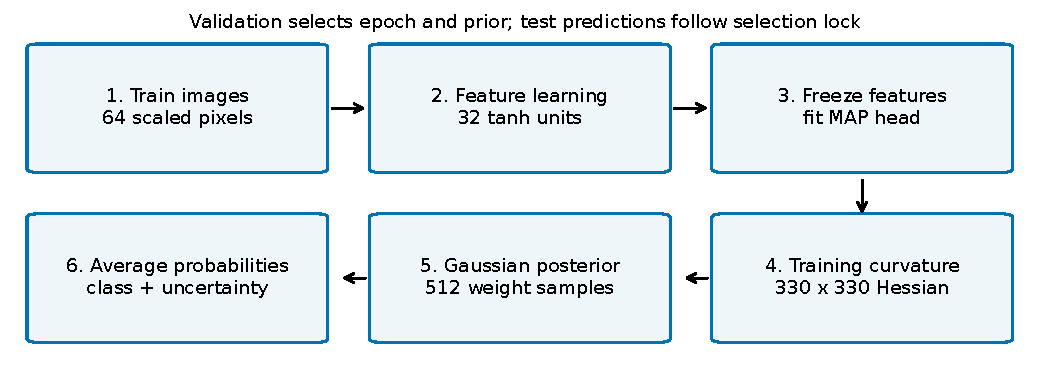
\includegraphics[width=\linewidth]{inference.pdf}
\caption{Implemented inference flow. Training supplies features and curvature;
validation selects checkpoints and $\alpha$. Test predictions follow the selection
record. Numbers and arrows specify the traversal order.}
\end{figure}

\subsection{Cost and limitations}
With $P=KD=330$, full Hessian storage is $O(P^2)$ and Cholesky factorization
is $O(P^3)$. Dense curvature accumulation costs $O(NK^2D^2)$ by direct
formulation, sampling costs $O(SP^2)$, and logits cost $O(SMKD)$ for $M$
evaluation images. Feature extraction is additional.
These costs scale poorly for very wide heads; full curvature is used here
for auditability.

The posterior is local and depends on the feature point estimate, Gaussian
prior and model specification. Monte Carlo probabilities have sampling error.
The model omits representation uncertainty. Selecting among three priors by
validation is not marginalization over $\alpha$ or marginal-likelihood
optimization. These project choices are distinct from the literature framework.


\section{How AI Implemented the Algorithm}
\subsection{Modules and equation-to-code mapping}
All experiment and reporting code was written by the AI agent. The authoritative
workflow is modular Python, without a notebook dependency. Configuration,
training, inference, evaluation and presentation are separated.
\begin{table}[H]\centering\small
\begin{tabularx}{\linewidth}{p{36mm}X}
\toprule File & Responsibility and mathematical connection\\\midrule
\texttt{data.py} & Images, fixed-range scaling, stratified split indices.\\
\texttt{features.py} & $h_\phi$, deterministic training, validation checkpoint.\\
\texttt{laplace.py} & Objective, gradient, Eq.~\ref{eq:hessian}, Cholesky draws.\\
\texttt{metrics.py} & Classification metrics, NLL, Brier, calibration bins.\\
\texttt{experiment.py} & Candidates, selection lock, final test predictions.\\
\texttt{figures.py} & Nine evidence figures and one tested toy geometry diagram.\\
\texttt{audit\_results.py} & Metrics, checkpoint reload and full-run verification.\\
\texttt{build\_report.py} & Numerical LaTeX tables generated from JSON.\\
\texttt{review\_diagnostics.py} & Fixed-model posterior sampling repetitions.\\
\bottomrule\end{tabularx}
\caption{Modules reside under \texttt{src/bayes\_digits/}, scripts under
\texttt{scripts/}.}
\end{table}
The head implementation is original project code, not a call to the paper's
\texttt{laplace} library. It implements one supported inference variant,
not every library feature or the paper's benchmarks.

\subsection{Executed pipeline pseudocode}
\begin{enumerate}[leftmargin=*,label=\arabic*.]
\item Load data, fix stratified indices, save configuration and dataset hash.
\item Fit Gaussian NB smoothing candidates on training images; select by validation NLL.
\item For each seed, train the image network for up to 120 epochs; retain the
checkpoint with minimum validation cross-entropy.
\item Freeze features. For each $\alpha\in\{0.1,1,10\}$, refit a MAP head,
check optimizer convergence and compute training-only posterior curvature.
\item Evaluate MAP and Laplace candidates on validation images; choose their
priors separately by minimum validation NLL.
\item Finish all seeds and write \texttt{selection\_locked.json}. Only then
transform test images and predict.
\item Evaluate primary models and the two predeclared frozen-prior ablations.
Save test probabilities, indices, labels, confusion matrices and metrics.
\item Generate plots and LaTeX tables; reload checkpoints and rerun the pipeline.
\end{enumerate}

\subsection{Checks, repairs and evidence}
Nine tests passed. They verify portable JSON evidence bytes, split coverage/disjointness, analytic derivatives
against independent PyTorch autograd, precision-to-covariance sampling,
normalization and serialization, known metric values and bin boundaries,
deterministic tiny-batch optimization, and rejection of invalid priors.
The binary example additionally checks the exact MAP and logit-contrast covariance.
The tiny-batch test achieves perfect training classification and loss below 0.02
on 20 images; repeated seeded feature training matches exactly.

The first test run failed while creating a Windows system temporary directory;
the serialization test had not executed. Moving pytest temporary files inside
the project resolved the access issue. A small end-to-end run with three feature
epochs executed before the full run. It selected its own models with validation
and evaluated after its selection lock; its test results were not used to change
the already specified full configuration. The audit then reloaded all primary
checkpoints, regenerated recorded metrics, and repeated the full pipeline.
All 18 saved arrays matched bit for bit in this environment.
Prompt 02 corrected loss logging: both training and validation NLL are now
evaluated after the completed epoch's optimizer update. Rerunning preserved
all 18 original prediction/label/index/MI arrays bit for bit against Git
snapshot \texttt{a28a563}; only the training-loss history and execution provenance
changed. The original results remain recoverable from that snapshot.


\section{Experiment Settings and Results}
\subsection{Dataset provenance and protocol}
The data are the \texttt{sklearn.datasets.load\_digits} copy of the UCI optical
handwritten digits dataset's 1,797-image \emph{test subset}
\cite{digits,skdigits}. The full UCI collection has a separate larger
training file, which this project does not use. These experiments repartition
the bundled subset; they are not results on UCI's original official protocol.
UCI records CC BY 4.0 usage conditions and a dataset DOI.

The images are available offline through scikit-learn, and the dataset is small
enough to verify full posterior matrices. Recognition uses flattened images
without augmentation, pretrained weights, PCA or fitted standardization.
Division by 16 follows the measurement range and fits no preprocessing
parameters on held-out images.

A stratified split holds out 20\% of all images with random state 3024.
A second stratified split holds out 25\% of the remainder using the same state.
Integer rounding gives 1,077 training, 360 validation and 360 test images.
Indices and per-class counts are saved. Test support ranges from 35 to 37
images per class. Figure~\ref{fig:data} uses those saved indices.
\begin{figure}[H]\centering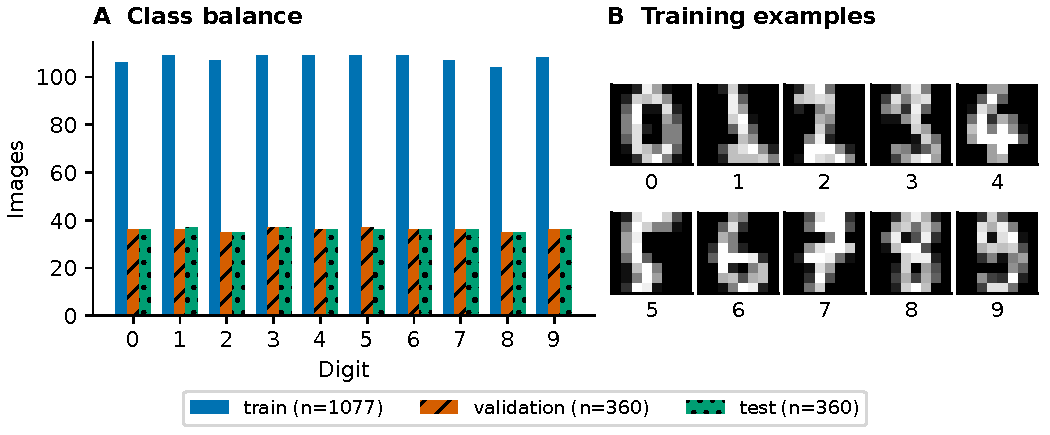
\includegraphics[width=\linewidth]{dataset.pdf}
\caption{Class counts by split and the first training image of each digit, enlarged in two rows.
The classes are nearly balanced. The range and nearest-neighbor display are fixed; examples are chosen
deterministically.}\label{fig:data}
\end{figure}

The evaluation unit is an image in this fixed subset. Writer identifiers are
not provided by the bundled loader, so writer-disjoint splitting is not
demonstrated. A new-writer deployment claim is unsupported. Three seeds describe
optimization variability conditional on one split; they do not turn 360
held-out images into 1,080 independent test examples.

\subsection{Research questions and controls}
The pre-execution questions were whether conditional last-layer inference
retains useful accuracy, whether posterior averaging improves probability
scores over a matched point predictor, and whether posterior correlations
matter. The frozen-prior MAP ablation isolates averaging at the same learned
representation and prior. The diagonal ablation isolates curvature structure
with the same mean, selected prior and sample count.

Gaussian NB is a simple statistical baseline with conditionally independent
Gaussian pixels and empirically estimated class priors:
\begin{equation}
p(y=k\mid x)\propto\frac{N_k}{N}\prod_{d=1}^{64}
\mathcal N(x_d;\mu_{kd},\sigma_{kd}^2+\epsilon),\quad
\epsilon=v\max_d\operatorname{Var}_{\rm train}(x_d).
\end{equation}
Class means and maximum-likelihood variances use training images only;
validation selects smoothing $v$. Normalized log-joint scores produce probabilities.
The selected $v=0.1$ stabilizes near-constant pixels. Spatial pixel
correlations challenge its assumptions. The separately tuned MAP head is a
discriminative comparison. All methods use identical partitions and a
validation-NLL selection rule. Equal architecture or search difficulty between
NB and the neural feature model is not assumed.


\subsection{Exact configuration and environment}
\begin{table}[H]\centering
\begin{tabularx}{\linewidth}{p{57mm}X}
\toprule Setting & Executed value\\\midrule
Input, classes & 64 pixels in $[0,1]$, ten classes\\
Feature network & Linear $64\rightarrow32$, tanh, linear $32\rightarrow10$ training head\\
Neural parameter count & 2,410 including biases\\
Initialization seeds; split seed & 11, 22, 33; 3024\\
Feature training & Adam, full training batch, learning rate 0.01\\
Feature decay; epoch budget & $10^{-4}$; 120 epochs\\
Checkpoint criterion & Minimum validation mean cross-entropy\\
Conditional head inference & SciPy L-BFGS-B, float64, max 2,000 iterations\\
Stopping options & \texttt{ftol} $10^{-14}$, \texttt{gtol} $10^{-7}$; gradient check $<10^{-3}$\\
Prior precision grid & 0.1, 1, 10; biases included\\
Gaussian NB smoothing grid & $10^{-9}$, $10^{-3}$, $10^{-1}$\\
Posterior prediction & 512 samples, full $330\times330$ Hessian\\
Calibration bins & Ten equal-width top-label confidence bins\\
Actual device; CPU threads & CPU; four PyTorch threads\\
Python; PyTorch & 3.12.14; 2.11.0+cu128\\
NumPy; SciPy; scikit-learn & 2.5.2; 1.18.1; 1.9.1\\
Operating system & Windows 11, build 26300\\
Detected GPU & NVIDIA GeForce RTX 5060 Ti; available but unused\\
\bottomrule\end{tabularx}
\caption{Configuration and observed environment. GPU availability does not
imply GPU execution. Complete provenance is in \texttt{environment.json}.}
\end{table}
CPU computation was chosen because this small full-batch problem and its dense
conditional Hessian are inexpensive. The review training/selection/evaluation
command took \RunSeconds\ seconds, excluding setup, tests, plotting and
compilation. This is one observed wall-clock duration, not a controlled hardware
benchmark. Existing PyTorch/scientific packages were reused read-only through
a local environment path; missing scikit-learn dependencies were installed in
the new Assignment 2 environment. README also gives a standalone setup recipe.

\begin{table}[H]\centering\begin{tabular}{rrrrr}\toprule
Seed & Feature epoch & MAP $\alpha$ & LA $\alpha$ & LA validation NLL \\\midrule
11 & 120 & 0.1 & 1 & 0.1516\\
22 & 120 & 0.1 & 1 & 0.1519\\
33 & 120 & 1 & 1 & 0.1648\\
\bottomrule\end{tabular}
\caption{Choices locked before full-run test predictions. All feature checkpoints
were selected at epoch 120. Laplace chose $\alpha=1$ for every seed.
Gaussian NB selected smoothing 0.1.}
\end{table}
The validation minimum at the budget boundary indicates that loss was still
improving over this range. The prespecified budget is reported rather than
increased in response to test results. Each prior candidate's validation NLL,
iterations and gradient residual is preserved. Full test probabilities permit
later audits without changing model choices.

\subsection{Evidence preservation}
The saved configuration, split indices, dataset hash, selection lock
and environment record identify the protocol.
\texttt{metrics.json}, \texttt{predictions.npz} and
\texttt{scalar\_metrics.csv} preserve numerical evidence.
Model files store the selected representation and conditional posterior.
Plot and table generators consume these saved files rather than embedded
hand-typed measurements.


\subsection{Metric definitions and overall results}
For $M=360$, accuracy is the proportion of correct argmax labels.
Class precision is $TP/(TP+FP)$, recall is $TP/(TP+FN)$, and
$F_1=2PR/(P+R)$, with zero when the relevant denominator vanishes.
Macro metrics average the ten class-specific values.
Laplace probability metrics use posterior-averaged probabilities:
\begin{align}
\mathrm{NLL}&=-\frac1M\sum_{i=1}^M\log \bar p_{y_i}(x_i),\\
\mathrm{Brier}&=\frac1M\sum_{i=1}^M\sum_{k=0}^{K-1}
(\bar p_k(x_i)-\mathbb{1}\{y_i=k\})^2.
\end{align}
Logs are natural, so NLL is in nats. NLL clips probabilities below $10^{-15}$.
Brier is summed over classes, not divided by ten; its range is $[0,2]$.
NLL of averaged probabilities differs from average sampled-head NLL.

For top-label calibration, confidence is $c_i=\max_k\bar p_k(x_i)$.
Let $B_b=\{i:b/10\leq c_i<(b+1)/10\}$, with the final bin also including $c_i=1$.
Then
\begin{equation}
\mathrm{ECE}=\sum_{b=0}^{9}\frac{|B_b|}{M}
|\mathrm{accuracy}(B_b)-\mathrm{confidence}(B_b)|.
\end{equation}
Empty bins contribute zero. This is a usual top-label calibration convention
\cite{guo}; ECE depends on binning and is not a proper scoring rule. NLL and
Brier carry more weight in evaluating probability quality.

\begin{table}[!htbp]\centering\small\begin{tabular}{lrrrr}\toprule
Method & Accuracy (\%) & Macro-F1 & NLL & Brier \\\midrule
Gaussian NB & 91.94 & 0.920 & 0.630 & 0.134\\
MAP & $97.78\pm 0.28$ & $0.978\pm 0.003$ & $0.099\pm 0.003$ & $0.040\pm 0.002$\\
Laplace & $97.69\pm 0.16$ & $0.977\pm 0.002$ & $0.151\pm 0.003$ & $0.055\pm 0.001$\\
\bottomrule\end{tabular}
\caption{Neural results are mean $\pm$ sample SD across three seeds.
The deterministic NB baseline was evaluated once. SD describes seed variability
on a shared test set, not a confidence interval.}
\end{table}
\begin{table}[!htbp]\centering\begin{tabular}{lrrr}\toprule
Method & Macro-precision & Macro-recall & ECE \\\midrule
Gaussian NB & 0.924 & 0.920 & 0.063\\
MAP & $0.978\pm 0.002$ & $0.978\pm 0.003$ & $0.017\pm 0.008$\\
Laplace & $0.977\pm 0.001$ & $0.977\pm 0.002$ & $0.080\pm 0.003$\\
\bottomrule\end{tabular}
\caption{Additional classification and calibration metrics.
Lower ECE is better under the specified ten-bin estimator.}
\end{table}
\begin{figure}[!htbp]\centering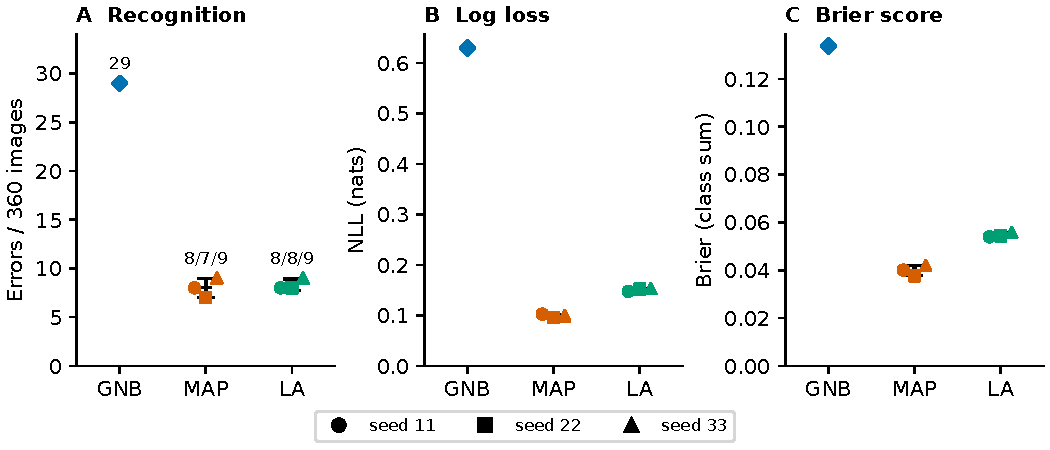
\includegraphics[width=\linewidth]{comparison.pdf}
\caption{Recognition error counts, NLL and class-summed Brier score; lower is better.
Horizontally offset shapes show each neural seed, black bars show mean $\pm$
sample SD, and GNB has one observation. All use the same 360 test images.
Axes start at zero. Neural methods make fewer errors than GNB, but MAP has
better probability scores than Laplace (LA).}
\end{figure}
The neural methods recognize digits more accurately than NB. MAP and Laplace
have similar accuracy, but MAP has lower NLL and Brier; Laplace ECE is higher.
The experiment therefore does not support improved probability quality from
this approximation. Accuracy alone would miss that result.
Small accuracy differences involve only a few images. No significance test or
statistical equivalence claim is made.


\subsection{Class-level results and feature training}
\begin{figure}[!htbp]\centering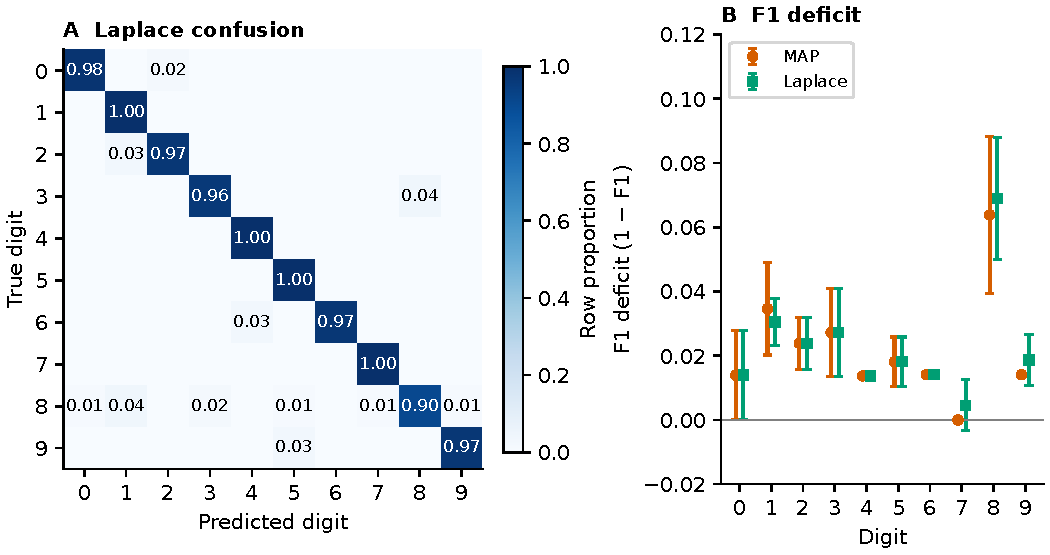
\includegraphics[width=\linewidth]{classes.pdf}
\caption{Laplace confusion is normalized by true-class support within each seed,
then averaged. Cell labels are percentages rounded to the nearest integer;
entries below 0.5\% are unlabeled. The color scale uses proportions.
The right panel plots
$1-F_1$ (lower is better) for every seed: filled MAP and open Laplace points,
with seed-specific shapes. Black dashes are means; vertical spans are the observed
min--max across three seeds, not SD bars or confidence intervals.
All observations remain visible on a nonnegative scale; Table~\ref{tab:class} gives raw F1.
Digit 8 is the weakest class. There are 360 unique test images.}
\end{figure}
\begin{table}[!htbp]\centering\begin{tabular}{rrrrr}\toprule
Digit & Test support & Precision & Recall & F1 \\\midrule
0 & 36 & 0.991 & 0.981 & 0.986\\
1 & 37 & 0.941 & 1.000 & 0.969\\
2 & 35 & 0.981 & 0.971 & 0.976\\
3 & 37 & 0.982 & 0.964 & 0.973\\
4 & 36 & 0.973 & 1.000 & 0.986\\
5 & 36 & 0.964 & 1.000 & 0.982\\
6 & 36 & 1.000 & 0.972 & 0.986\\
7 & 36 & 0.991 & 1.000 & 0.995\\
8 & 35 & 0.960 & 0.905 & 0.931\\
9 & 36 & 0.991 & 0.972 & 0.981\\
\bottomrule\end{tabular}
\caption{Mean Laplace per-class metrics across three seeds.
Support counts unique images, not three times that number.}
\label{tab:class}
\end{table}
Digit 8 has the weakest class F1 (0.931), with recall 0.905. Its averaged
mistakes are spread across several labels, including 1 and 3.
Digit 1 has perfect recall but lower precision because other digits are
sometimes assigned to it. Thus recall alone does not establish reliable
predictions of a label.
\begin{figure}[!htbp]\centering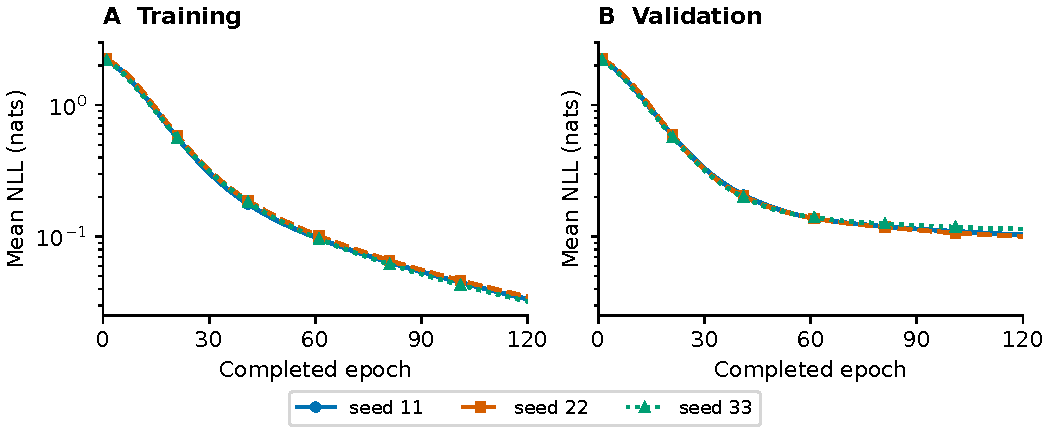
\includegraphics[width=\linewidth]{convergence.pdf}
\caption{Recorded feature-training and validation mean NLL on base-10 logarithmic axes.
Both panels share the same positive NLL limits and are evaluated after each epoch's optimizer update, using the original
training head before conditional MAP refitting. Line styles and markers identify
seeds. Loss continues to improve over the fixed budget; these curves do not
establish asymptotic convergence.}
\end{figure}
Both losses decrease through the prescribed budget. The curves do not prove
asymptotic feature-network convergence. Conditional head optimization is a
separate convex problem with checked gradient residuals; posterior inference
has no stochastic training trajectory in this implementation.


\subsection{Calibration, uncertainty and ablations}
\begin{figure}[!htbp]\centering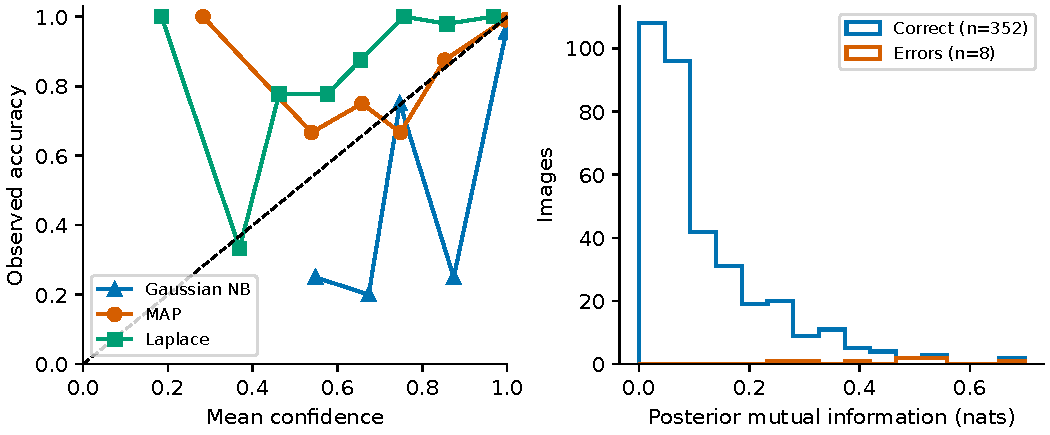
\includegraphics[width=\linewidth]{calibration.pdf}
\caption{Reliability and posterior mutual information for prespecified seed 11.
Ten equal-width confidence bins are used. Reliability points have equal size;
the aligned table gives every bin's image count, including zeros, for each method.
Empty-bin points are omitted and occupied points are not joined. Laplace is often underconfident,
but several bins contain few observations.
Right: empirical cumulative distributions normalized separately over 352 correct
and eight erroneous predictions. Errors often have greater disagreement, but
the distributions overlap and eight errors provide limited precision.}
\end{figure}
Several populated Laplace reliability bins lie above the identity line:
confidence is lower than observed success frequency. This agrees with higher
ECE/NLL, although sparse bins and only eight mistakes limit conclusions.
Many correct images have low posterior disagreement, while errors span a
broader range; within-group normalization exposes both distributions despite
their unequal sample counts. Overlap prevents a guaranteed error detector.
The representative seed was fixed before training.

\begin{table}[!htbp]\centering\begin{tabular}{lrrr}\toprule
Frozen-prior variant & Accuracy (\%) & NLL & ECE \\\midrule
Matched MAP & $97.69\pm 0.16$ & $0.097\pm 0.002$ & $0.025\pm 0.002$\\
Laplace & $97.69\pm 0.16$ & $0.151\pm 0.003$ & $0.080\pm 0.003$\\
Diagonal Laplace & $97.69\pm 0.42$ & $0.229\pm 0.0002$ & $0.147\pm 0.005$\\
\bottomrule\end{tabular}
\caption{Features and Laplace-selected prior are held fixed. Matched MAP removes
averaging; diagonal Laplace drops off-diagonal precision terms before inversion.
This differs from taking the diagonal of the full covariance.}
\end{table}
\begin{figure}[!htbp]\centering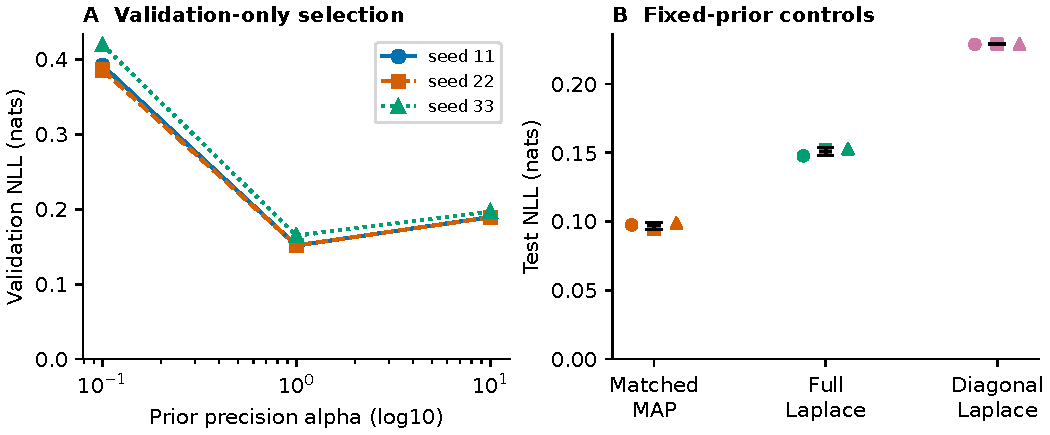
\includegraphics[width=\linewidth]{sensitivity.pdf}
\caption{Left: validation-only prior sensitivity. Right: predeclared frozen-prior
test NLL and seed SD, with offset seed points. $\alpha=1$ gives the lowest validation
NLL in this grid; full Laplace has lower test NLL than diagonal precision but
higher NLL than matched MAP. Test scores were not used to retune the prior.}
\end{figure}
Matched MAP has lower NLL than full Laplace with essentially identical aggregate
accuracy, isolating the effect of averaging rather than a different prior.
Diagonal Laplace increases NLL further. Keeping correlations improves this
approximation relative to the diagonal variant, but not relative to the
point estimate. Removing correlations can destroy cancellation of uncertain
common-logit directions. This mathematical explanation is compatible with
the results, not a separately measured causal decomposition.

Both $\alpha=0.1$ and $\alpha=10$ give worse Laplace validation NLL than
$\alpha=1$ for every seed. This demonstrates prior sensitivity within the
specified grid, not a globally optimal precision or an empirical-Bayes result.

\subsection{Post hoc Monte Carlo integration diagnostic}
Prompt 02 identified unmeasured sampling variation as a threat to interpreting
finite-sample predictions. The diagnostic held all selected features, heads,
priors and splits fixed; it did not perform model selection. Before executing
it, \texttt{configs/review\_diagnostics.json} specified sample counts
128/512/2048 and eight independent repetitions per model/count, giving
72 probability arrays on the same 360 test images. Sampling seed is
$2002000+10000r+10S+j$ for feature seed $r$, sample count $S$ and
repetition $j\in\{0,\ldots,7\}$. Repetition SD measures numerical integration
variation conditional on a fitted posterior, not test-set or retraining uncertainty.
\begin{figure}[!htbp]\centering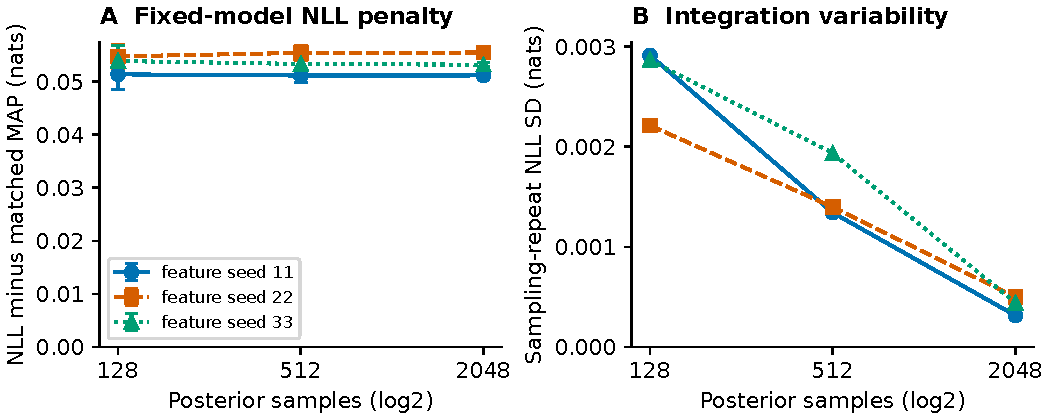
\includegraphics[width=\linewidth]{monte_carlo.pdf}
\caption{Post hoc fixed-model sampling diagnostic. Left: mean NLL penalty
against matched MAP with sampling-repeat SD, eight repetitions per point.
Right: the same SD alone. The penalty persists at 2048 samples while numerical
variation decreases; sampling noise alone does not account for the observed gap.
Models were not retuned and primary 512-sample results remain unchanged.}
\end{figure}
At 512 draws, within-model NLL SD across eight repetitions ranges from 0.0013 to 0.0019 nats. At 2048 draws, mean Laplace-minus-matched-MAP NLL remains 0.0511--0.0555 nats across the three fitted models. These descriptive results support a persistent probability-score penalty in this setting, rather than attributing it solely to the original random draws.

Independent repetitions sample the same approximate Gaussian, so this check
cannot establish the accuracy of the Laplace posterior approximation itself.


\subsection{Failure cases, interpretation and limits}
\begin{figure}[!htbp]\centering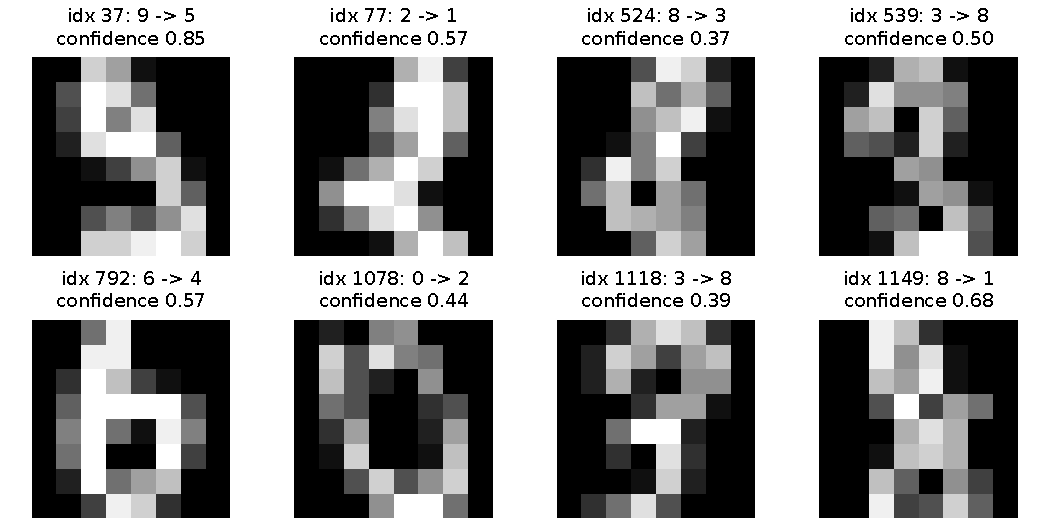
\includegraphics[width=\linewidth]{errors.pdf}
\caption{All eight Laplace errors for seed 11, ordered by original dataset index.
Titles show true digit, prediction and maximum posterior probability.
Native $8\times8$ pixels are displayed without smoothing.}
\end{figure}
Several mistakes involve ambiguous low-resolution strokes; that interpretation
is descriptive, not a measured explanation of image quality.
The 9-to-5 case has confidence 0.85, showing that a Bayesian predictor can still
make a relatively confident mistake. The 8-to-3 case has much lower confidence.
Selecting only favorable examples would conceal this variation.

\textbf{Answers to the research questions.} Conditional Laplace inference
retains high recognition accuracy in this experiment. It does not improve
the primary proper probability scores over independently selected MAP or the
matched-prior MAP control. Full covariance improves NLL over diagonal precision,
supporting attention to covariance structure rather than treating approximations
as interchangeable.

\textbf{Interpretation boundary.} One small, nearly balanced dataset, one split,
one architecture and three initialization seeds cannot establish a general
ranking of Bayesian classifiers. The Gaussian is local and omits representation
uncertainty. The prior grid is coarse and feature-scale dependent. Checkpoint
and prior selection reuse the same validation partition; there is no nested
validation estimate. The post hoc diagnostic quantifies integration variation
at three sample counts, but not uncertainty over representation or data sampling.
Writer independence, natural-image recognition, corruption and OOD detection
were not tested.

Prospective extensions include a wider validation-selected prior grid,
empirical-Bayes tuning, writer-separated
data or a second dataset. They were not executed and do not justify revising
the current conclusion using test outcomes. The negative calibration result
belongs in the evidence.

\textbf{Reproducibility.} \texttt{audit.json} verifies regenerated metrics,
checkpoint reloads and an identical full rerun. Tables read saved JSON;
figure provenance binds plots to source code and evidence. The original
execution hashes are preserved separately from revised plotting code.
These checks establish local reproducibility, not bitwise portability.
Unlike the large-network benchmarks in Laplace Redux \cite{laplace}, this study
uses a small head, frozen features and validation-grid prior selection.
The negative probability-quality result therefore evaluates this adaptation
and protocol, rather than refuting the paper's broader framework. The practical
lesson is to compare probability scores and numerical sensitivity alongside
recognition accuracy before drawing conclusions about uncertainty quality.


\FloatBarrier
\section{What I Have Learnt from This AI Assignment}
This assignment taught me that using an AI coding agent well is not just about asking it to write code. At the start, I thought the main challenge would be getting the agent to produce something that actually ran. But I quickly realized the harder part was giving it enough structure to keep the project on track. I used AGENTS.md to set the long-term rules: scientific integrity, reproducibility, mathematical rigor, experiment requirements, and report quality. Then I used smaller, task-specific Markdown prompts to break the work into stages: finding the algorithm, implementing it, running experiments, reviewing the results critically, and preparing the final report. That separation mattered. The permanent rules told the agent how the project should always behave, while the task prompts told it what to do next. I also learned that vague instructions lead to vague results. Clear requirements, constraints, and acceptance criteria made a real difference.

I also saw how specialized AI skills can raise the quality of the work. Instead of depending only on the model\textquoteright{}s general knowledge, I gave it skills for literature research, machine learning, PyTorch implementation, experimental design, statistical analysis, scientific visualization, and academic writing. The prompts explained what needed to be done, while the skills gave guidance on how to do it. The critical-review stage was especially useful. It pushed the agent to look back at its own results, find weak spots, improve the figures, and strengthen the technical explanations. Without that stage, I probably would have accepted the first report, even though it could have been much better.

Technically, the assignment deepened my understanding of Bayesian classification and uncertainty estimation. By studying the last-layer Laplace approximation, I saw how priors, likelihoods, and Bayes\textquoteright{} theorem connect to posterior inference. I also got a clearer picture of maximum a posteriori estimation, Hessian matrices, Gaussian posterior approximations, and Monte Carlo prediction. One point that I initially misunderstood was that computing an exact conditional Hessian does not make the posterior itself exact. The Laplace approximation is still a local Gaussian approximation, and it does not fully capture uncertainty in the learned feature representation.

Another lesson was that a more sophisticated algorithm does not always produce better results. The Laplace classifier reached about 97.69\% recognition accuracy, but its negative log-likelihood was higher than that of the MAP classifier. That result was humbling. It showed me that accuracy alone is not enough, especially for probabilistic models. Negative log-likelihood, Brier score, and calibration error tell us something important about whether the predicted probabilities can be trusted. I also learned to value controlled comparisons, repeated experiments, validation-based model selection, and careful error analysis. Even negative experimental findings can be useful if they are supported by evidence and explained clearly.

Overall, this assignment changed how I think about AI in programming and research. The quality of AI-generated work depends not only on how strong the model is, but also on how well the user organizes instructions, provides relevant skills, and defines verification standards. An AI agent can automate a lot of implementation, experimentation, and documentation, but I still need to understand the underlying concepts, question the methodology, and interpret the results. I now see AI as a powerful assistant, not a replacement for human judgment. Its usefulness depends on clear direction, reliable verification, and critical thinking.


\section{Webpage Link of the Source Codes}
GitHub publication and public wiki verification are deferred to Prompt 03;
no public URL exists yet. The earlier CLI authentication check reported an
invalid stored token. Source code and wiki pages are preserved locally in
\texttt{AI Assignment 2} and \texttt{docs/wiki/}, respectively.

\subsection*{Local reproduction}
After installing the pinned requirements, execute from the project root:
\begin{verbatim}
.\scripts\reproduce.ps1                 # PowerShell
.venv\Scripts\python.exe scripts/audit_results.py
.venv\Scripts\python.exe scripts/audit_review.py
\end{verbatim}
Compile \texttt{report/main.tex} with its tables and figures available.
The executed compiler was Tectonic 0.17.0 via the installed LaTeX plugin.
README includes standalone installation and compilation commands.
The generated PDF is rendered and reviewed page by page.

\begin{thebibliography}{9}\small\raggedright
\bibitem{laplace} E. Daxberger, A. Kristiadi, A. Immer, R. Eschenhagen,
M. Bauer and P. Hennig. \emph{Laplace Redux---Effortless Bayesian Deep Learning}.
NeurIPS 34, 2021.
\url{https://papers.nips.cc/paper/2021/hash/a7c9585703d275249f30a088cebba0ad-Abstract.html}.
\bibitem{natpn} B. Charpentier, O. Borchert, D. Z\"ugner, S. Geisler and
S. G\"unnemann. \emph{Natural Posterior Network: Deep Bayesian Uncertainty for
Exponential Family Distributions}. ICLR, 2022.
\url{https://arxiv.org/abs/2105.04471}.
\bibitem{vbll} J. Harrison, J. Willes and J. Snoek.
\emph{Variational Bayesian Last Layers}. ICLR, 2024.
\url{https://arxiv.org/abs/2404.11599}.
\bibitem{mackay} D. J. C. MacKay. \emph{Bayesian Interpolation}.
Neural Computation 4(3):415--447, 1992.
\url{https://doi.org/10.1162/neco.1992.4.3.415}.
\bibitem{digits} E. Alpaydin and C. Kaynak.
\emph{Optical Recognition of Handwritten Digits}. UCI dataset, 1998.
\url{https://doi.org/10.24432/C50P49}. CC BY 4.0.
\bibitem{skdigits} Scikit-learn documentation. \emph{load\_digits}.
Accessed 8 October 2026.
\url{https://scikit-learn.org/stable/modules/generated/sklearn.datasets.load_digits.html}.
\bibitem{guo} C. Guo, G. Pleiss, Y. Sun and K. Q. Weinberger.
\emph{On Calibration of Modern Neural Networks}. ICML, PMLR 70:1321--1330, 2017.
\url{https://proceedings.mlr.press/v70/guo17a.html}.
\bibitem{skills} T. Kassis, V. Agarwal, Y. He, D. Patel and A. M. Brueckner.
\emph{Scientific Agent Skills: A Library of Procedural Knowledge for Research Agents}.
ArXiv:2609.00065, 2026; record revised 2 September 2026.
\url{https://doi.org/10.48550/arXiv.2609.00065}.
\end{thebibliography}
\end{document}
